\chapter{配管6D姿勢推定}
本章では, 配管6D姿勢推定の手法について解説する. 
6D姿勢推定とは, 3次元空間内で物体の位置と姿勢を推定する技術であり, 深層学習の活用によりその効率と精度を大幅に向上させることが可能である. 
6D姿勢推定手法には入力データにRGB画像のみを用いる手法と, RGB-D画像を活用した手法の2種類がある. \\
 本章では, 以下の構成で解説を進める. 
第2.1節では, 検出対象である配管設備の特性を考慮し, 効率的なクラスの定義について述べる. 
第2.2節では, RGB画像を用いた配管の6D姿勢推定手法について説明する. 
第2.3節では, RGB-D画像を用いた配管の6D姿勢推定手法について解説する. 

\section{検出クラス}
深層学習による画像認識では, 検出対象となるオブジェクトを明確に定義することが重要である. 
検出対象のオブジェクトの名前はクラスと呼ばれ, それぞれのクラスに応じた学習が行われるのが一般的である. 
本研究では, 配管設備のアイソメ図を効率的に作成するために, 配管の構造的特徴を活用した手法を提案する. 

\begin{figure}[htbt]
	\centering
	 \includegraphics[height=52mm]{Figure/detect_class.eps}
	 \caption{配管構造の例}
	 \label{fig:2-f1}
\end{figure}

図\ref{fig:2-f1}に示すように, 一般的な配管は直管を中心とし, 接続部分として両端に曲管やT字管が存在する. 
この特性を利用し, 本研究では直管を検出対象から除外し, 接続部である曲管およびT字管の姿勢を推定する手法を採用した. 
これにより, 接続部同士のペアを直線で結ぶことで効率的にアイソメ図を描画することが可能である. \\
 さらに, 直管を検出対象に含める場合, 配管設備が大規模になるにつれて認識精度が低下することが問題となる. 
その主な要因は, オクルージョン問題にあり, 前方の配管が後方の配管を隠してしまうような状況では, 直管の認識が特に困難になる. \\
 以上の理由から, 本研究では検出対象のクラスを曲管とT字管の2種類に限定した. 
配管全体を解析するのではなく, これらの接続部に特化するアプローチを取ることで, 配管構造を効率的かつ正確に解析する手法を実現する. 

\section{RGB画像に基づく配管6D姿勢推定}
\subsection{全体構成}
RGB画像を用いた配管の6D姿勢推定には, Gen6Dを用いて実装する. 
図\ref{fig:2-f2}にGen6Dによる6D姿勢推定の流れを示す. 
\begin{figure}[htbt]
	\centering
	 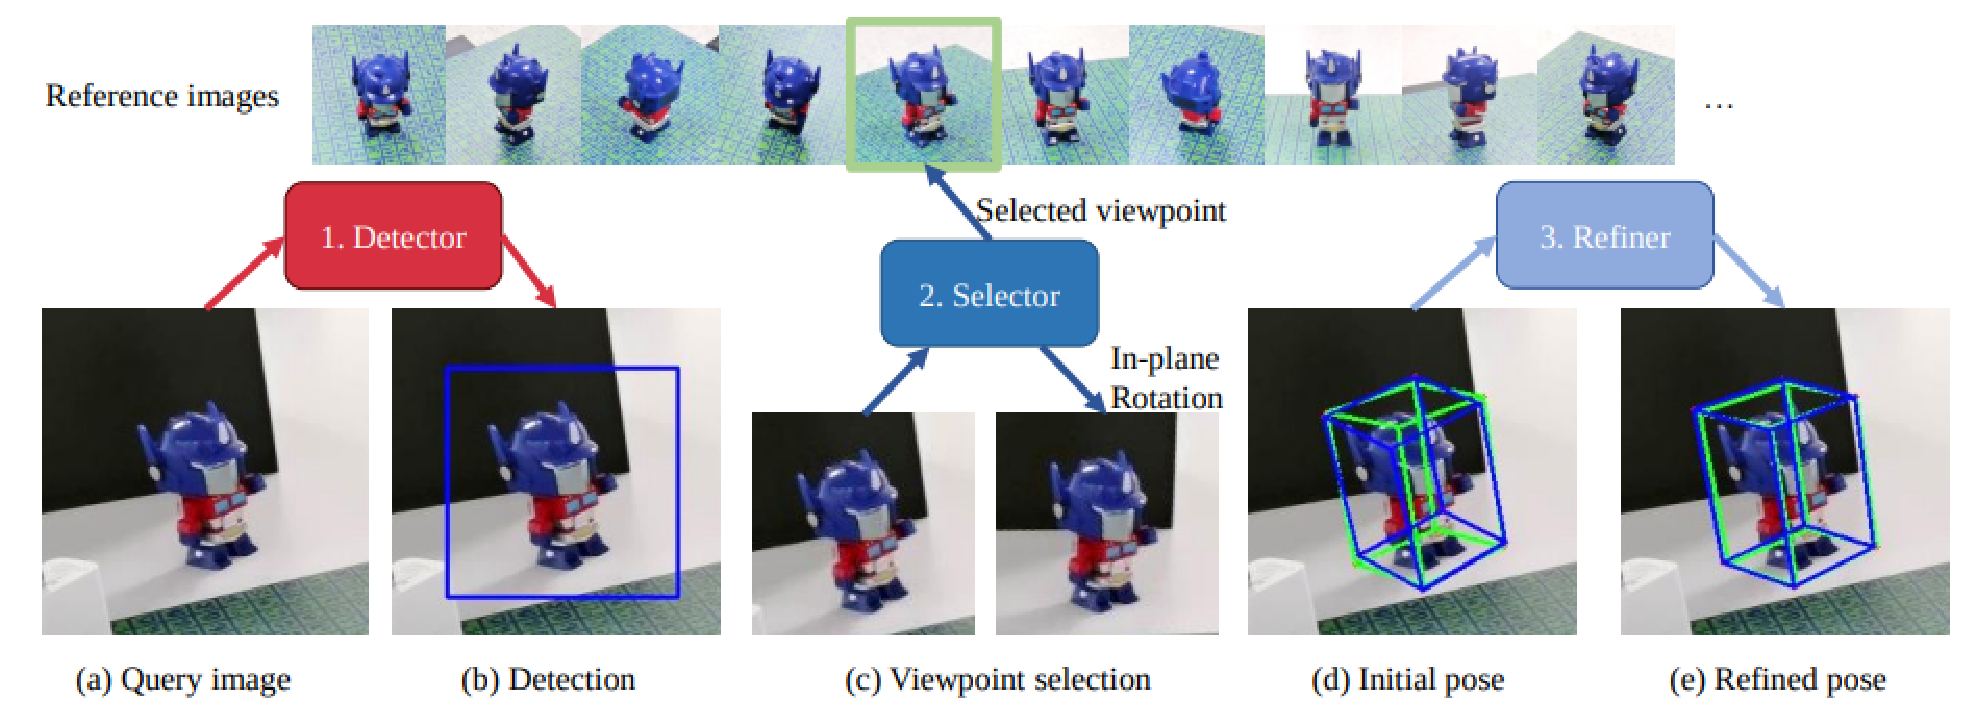
\includegraphics[height=45mm]{Figure/Gen6D.eps}
	 \caption{Gen6Dの姿勢推定方法の流れ}
	 \label{fig:2-f2}
\end{figure}

Gen6DはDetector(物体検出), Selector(画像マッチング), Refiner(姿勢補正)の3つのステップから構成されている. 
物体検出では, 入力画像から対象物体の領域を検出し, 画像マッチングでは, 検出された領域を参照画像と比較して最も類似する視点を持つ画像を選択する. 
姿勢補正では, 初期姿勢を基に, 複数の参照画像を利用して6D姿勢情報をさらに精度良く推定する. \\
 しかし, Gen6Dは単一物体の姿勢推定に特化しており, 複数物体を同時に処理することが困難である. 
このため, 複数の配管部品を含むアイソメ図を作成する際には, 複数物体を同時に検出可能な手法が求められる. 
一方で, YOLOは各検出クラスに対して複数物体の検出が可能であり, Gen6Dの物体検出ステップの代替手法として有効である. \\
 本研究では, YOLOを用いて各接続部を検出し, その結果を基にGen6Dを用いて姿勢を推定する手法を提案する. 
データ収集から配管6D姿勢推定までの全体的な流れを図\ref{fig:2-f3}に示す. 
\begin{figure}[htbt]
	\centering
	 \includegraphics[height=52mm]{Figure/RGB_flow.eps}
	 \caption{RGB画像に基づく配管6D姿勢推定の流れ}
	 \label{fig:2-f3}
\end{figure}


\subsection{物体検出}
YOLOのアルゴリズムでは, 図\ref{fig:2-f4}に示すように入力画像を $S \times S$ のグリッドセルに分割し, 各セルで複数のバウンディングボックスとその信頼度を計算する. \\
\begin{figure}[htbt]
	\centering
	 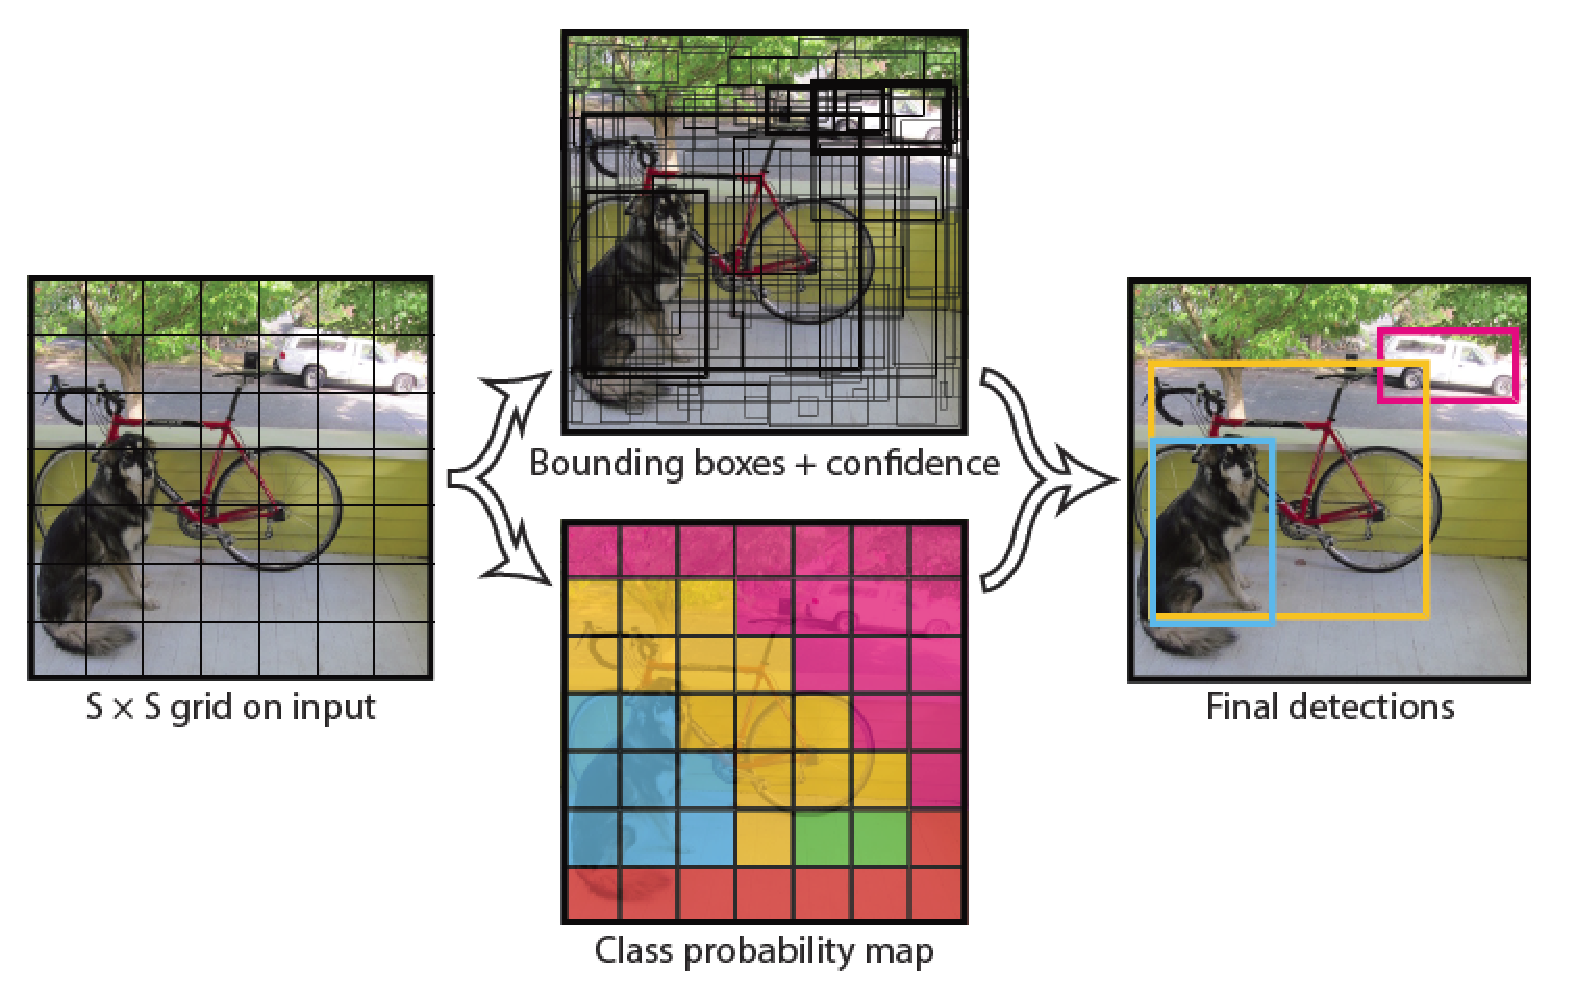
\includegraphics[height=75mm]{Figure/YOLO.eps}
	 \caption{物体検出YOLOの検出アルゴリズム}
	 \label{fig:2-f4}
\end{figure}
 物体の中心が特定のグリッドセル内に位置する場合, そのセルは物体を検出するように学習される. 
その後, 各セルでバウンディングボックスが推定され, $B$個のバウンディングボックスに対してそれぞれ信頼スコアが予測される. 
この信頼スコアは, 特定のバウンディングボックスが物体を含む確率と, その精度を示す指標となる. \\
 次に, YOLOの損失関数について説明する. 損失関数はネットワークの出力と正解ラベルとの誤差を計算する役割を担い, その最小化によってモデルの学習が進む. 
損失関数は式(2.1)に示すように, 物体の中心座標, バウンディングボックスの幅と高さ, 物体の存在確率, クラス予測という4つの項目の誤差から構成される. 

\begin{align*}
	\text{Loss} = 
	&\ \lambda_{\text{coord}} \sum_{i=0}^{S^2} \sum_{j=0}^{B} 1^{\text{obj}}_{ij} 
	\left[ (x_i - \hat{x}_i)^2 + (y_i - \hat{y}_i)^2 \right] \\
	&+ \lambda_{\text{coord}} \sum_{i=0}^{S^2} \sum_{j=0}^{B} 1^{\text{obj}}_{ij} 
	\left[ (2 - w_i \cdot h_i) \left[ (w_i - \hat{w}_i)^2 + (h_i - \hat{h}_i)^2 \right] \right] \\
	&- \sum_{i=0}^{S^2} \sum_{j=0}^{B} 1^{\text{obj}}_{ij} 
	\left[ \hat{C}_i \log(C_i) + (1 - \hat{C}_i) \log(1 - C_i) \right] \\
	&- \lambda_{\text{noobj}} \sum_{i=0}^{S^2} \sum_{j=0}^{B} (1 - 1^{\text{obj}}_{ij}) 
	\left[ \hat{C}_i \log(C_i) + (1 - \hat{C}_i) \log(1 - C_i) \right] \\
	&- \sum_{i=0}^{S^2} 1^{\text{obj}}_i \sum_{c \in \text{classes}} 
	\left[ \hat{p}_i(c) \log(p_i(c)) + (1 - \hat{p}_i(c)) \log(1 - p_i(c)) \right]
	\tag{2.1}
\end{align*}

ここで, $S^2$ はグリッドセルの総数を表し, $B$ は各グリッドセルで予測されるバウンディングボックスの数を示す. 
また, $\lambda_{\text{coord}}$ と $\lambda_{\text{noobj}}$ は, それぞれ座標損失と物体が存在しない場合の信頼度損失に対応する重み付けパラメータを示す. 
$(x_i, y_i)$ および $(w_i, h_i)$ は, バウンディングボックスの中心座標と幅・高さを示し, 一方で $(\hat{x}_i, \hat{y}_i)$ および $(\hat{w}_i, \hat{h}_i)$ は, これらの推定値である. 
$C_i$ および $\hat{C}_i$ は, 物体が存在する信頼度スコアの真値と推定値を表す. 
さらに, $p_i(c)$ および $\hat{p}_i(c)$ は, クラス $c$ に関する真値と推定値としてのクラス確率を意味する. 
この損失関数は, 検出精度を向上させるため, バウンディングボックスの位置とサイズの精度, およびクラス予測の精度を考慮している. 

\subsection{画像マッチング}
画像マッチングでは, 物体検出によって得られた画像に最も近い視点を持つ参照画像を選択することを目的とする. 
参照画像は, Colmapを活用して内部パラメータおよび外部パラメータを取得することが可能である. 
これにより, テスト画像に最も類似した参照画像の視点情報を基に, 物体の初期姿勢を推定することが可能となる. 
画像マッチングのアーキテクチャを図\ref{fig:2-f5}に示す. 
\begin{figure}[htbt]
	\centering
	 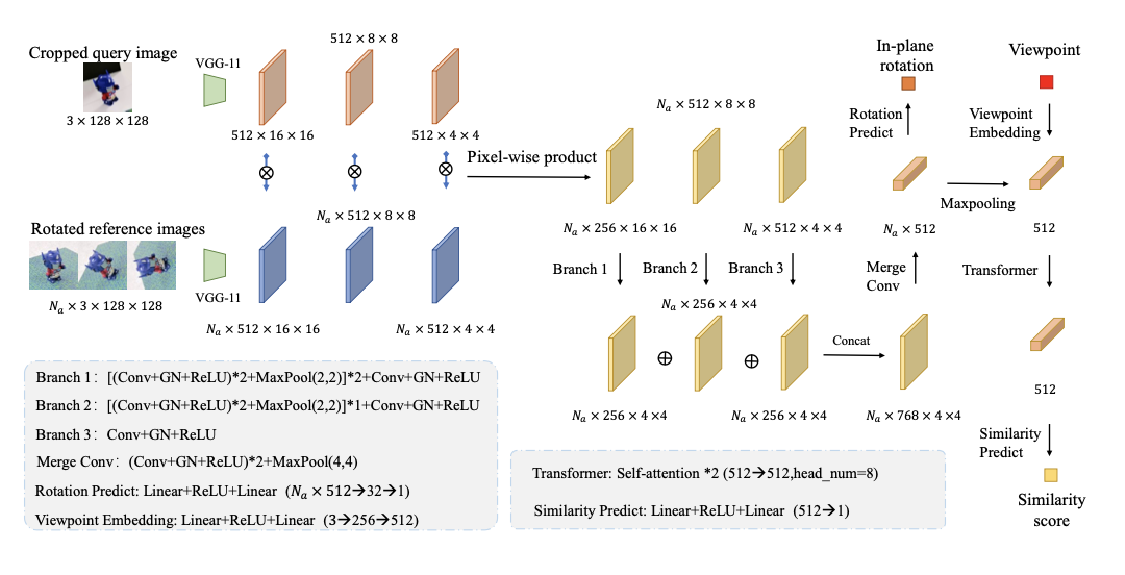
\includegraphics[height=72mm]{Figure/selector_arc.eps}
	 \caption{画像マッチングのアーキテクチャ}
	 \label{fig:2-f5}
\end{figure}

このプロセスは, まずVGG-11という深層学習モデルを用いて入力画像および参照画像から特徴マップを抽出する. 
その後, 入力画像と各参照画像の特徴マップをピクセル単位で相関させ, スコアマップを生成する. 
この計算により, 物体領域の類似性が強調され, 背景などのノイズの影響を効果的に抑制することができる. \\
 次に, 参照画像全体の特徴分布を正規化するグローバル正規化が適用される. 
この正規化により, 参照画像間の相対的な類似性が明確化され, ノイズの影響が軽減される仕組みである. 
その後, Transformerと呼ばれる深層学習モデルが用いられる. 
Transformerとは, 自己注意メカニズム(self-attention)を通じて参照画像間の情報を共有し, 文脈を考慮した類似度スコアを算出するモデルのことである. 
このスコアに基づき, 最大スコアを持つ参照画像が入力画像に最も近い視点を持つ画像として選択される. \\
 画像マッチングのトレーニングには式2.2に示した類似度損失が使用される. 
この損失は, 入力画像と参照画像のカメラ位置ベクトルを正規化し, 内積を用いて視点類似度を計算するものである. 
計算された視点類似度を正解値として, 予測スコアとの間のバイナリ交差エントロピー損失を最小化する. 
\begin{equation}
	\ell_{\text{sim}} = \sum_{i} - \left( \tilde{s}_i \log(s_i) + (1 - \tilde{s}_i) \log(1 - s_i) \right)
	\tag{2.2}
\end{equation}
	
ここで, \(\tilde{s}_i\)はスケーリングされた視点類似度の正解値, \(s_i\)はモデルによって予測された類似度スコアを表す. 

\subsection{姿勢補正}
Gen6Dの姿勢補正は, 初期推定された物体の姿勢を精密化するために設計された手法であり, 特にモデルフリーの状況において高い汎用性を発揮する. 
姿勢補正のアーキテクチャを図\ref{fig:2-f6}に示す. 
\begin{figure}[htbt]
	\centering
	 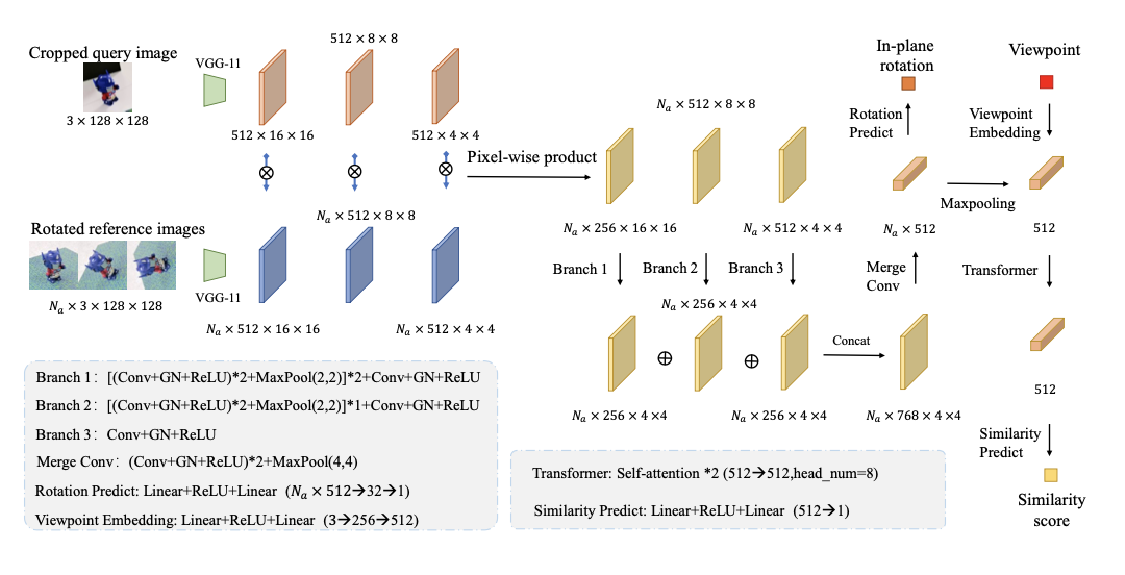
\includegraphics[height=72mm]{Figure/selector_arc.eps}
	 \caption{姿勢補正のアーキテクチャ}
	 \label{fig:2-f6}
\end{figure}

基本的なアプローチとして, Gen6Dは参照画像の情報を3D空間に統合し, それを解析することで精密な6D姿勢を推定する. 
まず, 入力された初期姿勢に基づき, その姿勢に近い複数の参照画像を選択する. 
選択された参照画像の特徴量は3D空間に逆投影され, 特徴ボリュームが構築される. 
同時に, テスト画像から抽出された特徴量も3D空間に投影され, 参照画像の特徴量と結合される. 
この手法により, 対象物の特徴を反映した3Dボリュームが生成される. \\
 生成された3Dボリュームに対しては, 3D畳み込みニューラルネットワーク(3D CNN)が適用される. 
3D CNNは空間的な情報を効果的に解析可能なニューラルネットワークであり, 特徴マップを解析することで初期推定された粗い姿勢に対する残差を予測する. 
これにより, 最終的に精密な6D姿勢が得られる. 
従来手法では, 姿勢精密化の過程でレンダリングを用いてテスト画像との比較を行うことが一般的であったが, Gen6Dの姿勢補正ではこのようなレンダリング工程を必要としない. 
この点が, モデルフリーな環境で特に有効であり, 未知の物体や環境に対しても高い精度を実現する要因となっている. \\
 最後に, 損失関数はサンプリングされた点群を用いて予測された姿勢と正解の姿勢の間の差を最小化するものが用いられる. 

\begin{equation}
\mathcal{L}_{\text{ref}} = \sum_{k} \|s_{\text{pr}} R_{\text{pr}} (p_k + t'_{\text{pr}}) - s_{\text{gt}} R_{\text{gt}} (p_k + t'_{\text{gt}})\|^2
\tag{2.3}
\end{equation}

ここで, \(p_k\)は入力カメラ座標系におけるサンプリング点, \(s_{\text{pr}}, R_{\text{pr}}, t'_{\text{pr}}\)はそれぞれ予測されたスケール, 回転, 平行移動, \(s_{\text{gt}}, R_{\text{gt}}, t'_{\text{gt}}\)は正解のスケール, 回転, 平行移動を示す. 


\section{RGB-D画像に基づく配管6D姿勢推定}
\subsection{全体構成}
RGB-D画像を用いた配管の6D姿勢推定には, SAM-6Dを使用して実装する. 
図\ref{fig:2-f7}にSAM-6Dによる6D姿勢推定の流れを示す. 
\begin{figure}[htbt]
	\centering
	 \includegraphics[height=90mm]{Figure/SAM-6D.eps}
	 \caption{SAM-6Dによる6D姿勢推定の流れ}
	 \label{fig:2-f7}
\end{figure}

SAM-6Dは, インスタンスセグメンテーションとしてSegment AnythingとObject Matchingを活用し, 姿勢推定の段階ではCoarse Point Matching(ポイントマッチング)とFine Point Matching(姿勢補正)のステップを経て6D姿勢を推定するモデルである. 
SAM-6Dはインスタンスセグメンテーションにおいて事前学習データを基にゼロショットで推論や予測を行うことが可能なモデルである. 
しかし, 本研究では検出対象のクラスが事前に定義されているため, Segment Anythingの汎用的なセグメンテーション機能は使用せず, Object Matchingを用いてインスタンスセグメンテーションを行う. 
よって, RGB-D画像に基づく配管6D姿勢推定は図\ref{fig:2-f8}のようになる. 
\begin{figure}[htbt]
	\centering
	 \includegraphics[height=57mm]{Figure/RGB-D_flow.eps}
	 \caption{RGB-D画像に基づく配管6D姿勢推定の流れ}
	 \label{fig:2-f8}
\end{figure}

\subsection{インスタンスセグメンテーション}
セグメンテーションは, 画像からピクセル単位で対象物体を認識する手法であり, 物体検出がバウンディングボックスの取得に留まるのに対し, より正確に物体の形状を特定できる. 
それに加え, インスタンスセグメンテーション(ISM)は複数の物体を同時に検出し, それぞれに異なるをラベルを付与することが可能である. 
画像内の配管接続部全てに対しての6D姿勢情報が必要になるため, インスタンスセグメンテーションを用いて配管接続部の検出を行う. 
SAM-6DのISMではSemantics, Appearance, Geometryの3つの情報が抽出される. \\
 Semantic Scoreは, 提案領域とテンプレートのセマンティックな一致度を評価するスコアである. 
提案領域とテンプレートのクラス埋め込み間の内積を用いて計算される. 
このスコアでは, $f^{cls}_{Im}$ は提案領域 $Im$ のクラス埋め込みを, $f^{cls}_{T_k}$ はテンプレート $T_k$ のクラス埋め込みをそれぞれ表し, テンプレート数を $N_T$ として計算される. 
\[
s_{sem} = \left\{ \frac{\langle f^{cls}_{Im}, f^{cls}_{T_k} \rangle}{|f^{cls}_{Im}||f^{cls}_{T_k}|} \right\}_{k=1}^{N_T}
\]
 Appearance Scoreは, 提案領域とテンプレートの外観の類似度を評価するスコアである. 
このスコアは, 提案領域内の各パッチ埋め込みとテンプレート内の各パッチ埋め込み間の最大類似度を基準に計算される. 
ここで, $f^{\text{patch}}_{Im,j}$ は提案領域のパッチ $j$ の埋め込みを, $f^{\text{patch}}_{T_{\text{best}},i}$ は最もマッチしたテンプレートのパッチ $i$ の埋め込みをそれぞれ表し, 提案領域のパッチ数を $N_{Im}^{\text{patch}}$ , テンプレートのパッチ数を $N_{T_{\text{best}}}^{\text{patch}}$ として以下の式で計算される. 
\[
s_{appe} = \frac{1}{N_{Im}^{\text{patch}}} \sum_{j=1}^{N_{Im}^{\text{patch}}} \max_{i=1, \dots, N_{T_{\text{best}}}^{\text{patch}}} \frac{\langle f^{\text{patch}}_{Im,j}, f^{\text{patch}}_{T_{\text{best}},i} \rangle}{|f^{\text{patch}}_{Im,j}| |f^{\text{patch}}_{T_{\text{best}},i}|}
\]
 Geometric Scoreは, 提案領域とテンプレートの幾何学的類似性を評価するスコアである. 
このスコアは, 提案領域のバウンディングボックスと, 粗いポーズ推定によって変換されたオブジェクトの投影バウンディングボックスのIoU(Intersection-over-Union)によって計算される. 
ここで, $B_m$ は提案領域のバウンディングボックスを, $B_o$ は変換されたオブジェクトのバウンディングボックスをそれぞれ表し, 以下の式で計算される. 
\[
s_{geo} = \frac{B_m \cap B_o}{B_m \cup B_o}
\]
 さらに, 可視性比率(Visible Ratio, $r_{vis}$)を用いてスコアの信頼性を調整する. 
最終的なObject Matching Scoreは, 上記の3つのスコアを統合して以下の式で計算される
\[
s_m = \frac{s_{sem} + s_{appe} + r_{vis} \cdot s_{geo}}{1 + 1 + r_{vis}}
\]


\subsection{姿勢推定}
図\ref{fig:2-f9}にSAM-6Dによるポイントマッチングおよび姿勢補正の流れを示す. 
\begin{figure}[htbt]
	\centering
	 \includegraphics[height=82mm]{Figure/SAM-6D_pose_flow.eps}
	 \caption{SAM-6Dのポイントマッチングおよび姿勢補正の流れ}
	 \label{fig:2-f9}
\end{figure}

Coarse Point Matchingは, 提案物体点群と対象物点群間で初期的な対応関係を確立し, 対象物の粗い6Dポーズを推定する手法である. 
この方法は, 提案物体点群$P_m$と対象物点群$P_o$からそれぞれ疎なサブセット$P_m^c \in \mathbb{R}^{N_m^c \times 3}$および$P_o^c \in \mathbb{R}^{N_o^c \times 3}$をサンプリングし, それらの間で対応付けを行う. 

まず, 提案物体点群と対象物点群それぞれの疎点群に対応する特徴量行列$F_m^c \in \mathbb{R}^{N_m^c \times C}$および$F_o^c \in \mathbb{R}^{N_o^c \times C}$を計算する. 
ここで, 学習可能な背景トークン$f_{\text{bg}, m}^c \in \mathbb{R}^C$および$f_{\text{bg}, o}^c \in \mathbb{R}^C$を特徴量行列に付加する. 
この背景トークンは, 提案物体点群と対象物点群の間に対応する点が存在しない場合, 未対応の点を処理するために導入されている. 
特徴量行列を用いて, 以下のようにアサインメント行列$A^c$を計算する. 

\[
A^c = [f_{\text{bg}, m}^c, F_m^c] \cdot [f_{\text{bg}, o}^c, F_o^c]^T
\]

このアサインメント行列は, 提案物体点群の各点が対象物点群のどの点と対応しているか, または背景トークンと対応しているかを示すスコアを表す. 
この行列を正規化することで, ソフトアサインメント行列$\tilde{A}^c$を導出する. 

\[
\tilde{A}^c = \text{Softmax}_{\text{row}}\left(\frac{A^c}{\tau}\right) \cdot \text{Softmax}_{\text{col}}\left(\frac{A^c}{\tau}\right)
\]

ここで, $\tau$は温度パラメータであり, 値を調整することで確率分布の滑らかさを制御する. 
ソフトマックス操作により, 行列内の各値は0から1の範囲に正規化され, 行方向および列方向でそれぞれの合計が1になるように処理される. 
ソフトアサインメント行列$\tilde{A}^c$を用いて, 提案物体点群と対象物点群間の対応点ペアを抽出する. 
これに基づいてポーズ仮説$(R_{\text{hyp}}, t_{\text{hyp}})$を生成する. 仮説ポーズの評価には以下のスコア関数を用いる. 

\[
s_{\text{hyp}} = \frac{N_m^c}{\sum_{p_m^c \in P_m^c} \min_{p_o^c \in P_o^c} \| R_{\text{hyp}}^T (p_o^c - t_{\text{hyp}}) - p_m^c \|_2 }
\]

このスコア$s_{\text{hyp}}$は, 提案物体点群と対象物点群間の対応精度を定量化しており, 最も高いスコアを持つ仮説ポーズ$(R_{\text{hyp}}, t_{\text{hyp}})$が初期ポーズ$(R_{\text{init}}, t_{\text{init}})$として選択される. 

\subsection{姿勢補正}
姿勢補正では画像マッチングによって推定された粗いポーズをさらに精緻化する手法である. 
姿勢補正は, 提案領域とテンプレートの点群セット間で密な対応を構築し, より正確な物体のポーズを推定するプロセスである. 
このプロセスでは, 初期姿勢推定結果を使用して, 点群の座標を変換し, 位置エンコーディングを学習する. 具体的には, 以下の手順で進行する. \\
 まず, 提案領域の点群 $P_m$ から高密度の点群セット $P_m^f \in \mathbb{R}^{N_m^f \times 3}$ をサンプリングし, 同様にテンプレートの点群 $P_o$ から $P_o^f \in \mathbb{R}^{N_o^f \times 3}$ をサンプリングする. 
ここで, $N_m^f$ および $N_o^f$ はそれぞれ高密度点群の点数である. 
次に, 粗いポーズ推定結果である $R_{init}$ および $t_{init}$ を用いて, 提案領域の点群 $P_m^f$ を変換し, 
\[
P_m^{f, \text{transformed}} = R_{init} P_m^f + t_{init}
\]
とする. この変換結果に基づいて, 位置エンコーディングを学習する. 位置エンコーディングは, 点群の幾何学的な位置関係を特徴空間に埋め込むために使用される. \\
 その後, Sparse-to-Dense Point Transformer(SDPT)を用いて, 高密度点群間の対応関係を学習する. 
SDPTでは, まず低密度な特徴をサンプリングし, それらの特徴間の関係を学習した後, それを高密度な特徴に拡張する. 
このプロセスにより, 効率的かつ効果的に高密度点群間の対応を確立できる. 
最終的に, 学習された対応関係に基づいて, 以下の式で物体の最終的なポーズ $R$ および $t$ を推定する.
\[
(R, t) = \text{Weighted SVD}(P_m^f, P_o^f)
\]
ここで, Weighted SVD は対応点間の重み付き特異値分解を指す. 
この結果により, 初期姿勢をより精緻化した姿勢を推定することが可能となる. 
